%%%%%%%%%%%%%%%%%%%%%%%%%%%%%%%%%%%%%%%%%%%%%%%%%%%%%%%%%%%%%%%%%%%%%%%%
% Plantilla TFG/TFM
% Escuela Politécnica Superior de la Universidad de Alicante
% Realizado por: Jose Manuel Requena Plens
% Contacto: info@jmrplens.com / Telegram:@jmrplens
%%%%%%%%%%%%%%%%%%%%%%%%%%%%%%%%%%%%%%%%%%%%%%%%%%%%%%%%%%%%%%%%%%%%%%%%

\chapter{Teoría de Antenas}
\par En este capitulo se realizará una breve contextualización sobre el concepto de antena así como un repaso a los parámetros que las caracterizan. Estos conceptos son, por lo general, aplicables a cualquier tipo de antena, en capítulos posteriores se especificará lo aprendido para el caso de las antenas en tecnología microstrip.

\section{Conceptos básicos}

\par Las antenas son transductores entre un medio guaiado y uno radiado. En su diseño más simplificado se analizaría un conductor metálico por el cual fluye una corriente variable en el tiempo. Se entiende como medio guiado a cualquier tipo de línea de transmisión: Cable coaxial, fibra óptica así como guías de onda. Y como medio radiado el aire o el espacio. Las antenas transmisoras serán las encargadas de transformar esta las corrientes eléctricas a \gls{oem}, mientras que las receptoras tomarán las \gls{oem} desde el medio radiado y las convertirán de nuevo a impulsos eléctricos para su posterior procesado. Las primeras antenas fueron diseñadas en 1888 por \textit{Heinrich Hertz} pero no fue hasta 1895 cuando \textit{Guglielmo Marconi} empezó a desarrollar antenas con el objetivo de transmitir información a largas distancias.
\\
\par Como se explico en el \todo{capitulo1}, cualquier variación de un campo eléctrico generará un campo magnético y viceversa. Cuando ambos campos conviven y existen variaciones de estos campos se dice que existe una radiación electromagnética. Para entender el principio de funcionamiento de una antena se tomará como ejemplo el caso de hilo conductor cerrado. Si se introdujera una corriente eléctrica fluctuante en el tiempo dentro del conductor, por el principio de inducción electromagnética (Tercera ecuación de Maxwell, Ley de Faraday-Lentz) se produciría un campo magnético fluctuante y un campo eléctrico asociado a su alrededor, estaríamos hablando de un campo electromagnético. Pero este campo electromagnético no se propagaría y estaría siempre al rededor del conductor cerrado. Para poder propagar las \gls{oem} se debe conseguir separar la onda electromagnética del conductor.
\\
\par Para entender el efecto de separación se tomará como referencia dos cargas eléctricas de distintas polaridades separadas a una distancia determinada (fig. \ref{fig:campo1}), a esto se le conoce como dipolo eléctrico y producirán un campo eléctrico cuyas líneas de fuerza irán del positivo al negativo. Estás dos cargas intentarán juntarse debido al efecto de atracción. En el momento de mayor separación de las cargas, su velocidad será nula y su aceleración máxima. Conforme se vayan acercando la velocidad irá aumentando y la aceleración disminuyendo hasta que en el punto donde se encuentran la velocidad será máxima y la aceleración nula. Suponiendo un escenario teórico sin pérdidas estás cargas estarían fluctuando e intercambiando sus posiciones indefinidamente. Si se analiza el campo eléctrico producido por las cargas mientras estas están fluctuando se observaría como, en vez de seguir encontrando un campo eléctrico simple de menor intensidad, este se deforma debido a la aceleración presente en las cargas. Esta deformación es también conocida como efecto \textit{kink} (fig. \ref{fig:campo2}).
\\
\par Continuando con el experimento se observa como pasado un lapso de un 1/4 del periodo de la oscilación, momento en el que las dos cargas se cruzan en el mismo punto, el campo eléctrico producido es nulo, cerrándose así las líneas de campo que habían sido producidas cuando las partículas estaban aún separadas (fig. \ref{fig:campo3}). Es entonces cuando se produce la propagación y generación del frente de onda del campo eléctrico, con su respectivo campo magnético asociado. Se debe observar como la longitud de la \gls{oem} propagada es exactamente el doble de la longitud existente entre las dos cargas (fig. \ref{fig:campo4}).\\

\begin{figure}[h]
\centering
	\begin{subfigure}[b]{0.3\textwidth} % Espacio horizontal ocupado por la subfigura
		\centering
		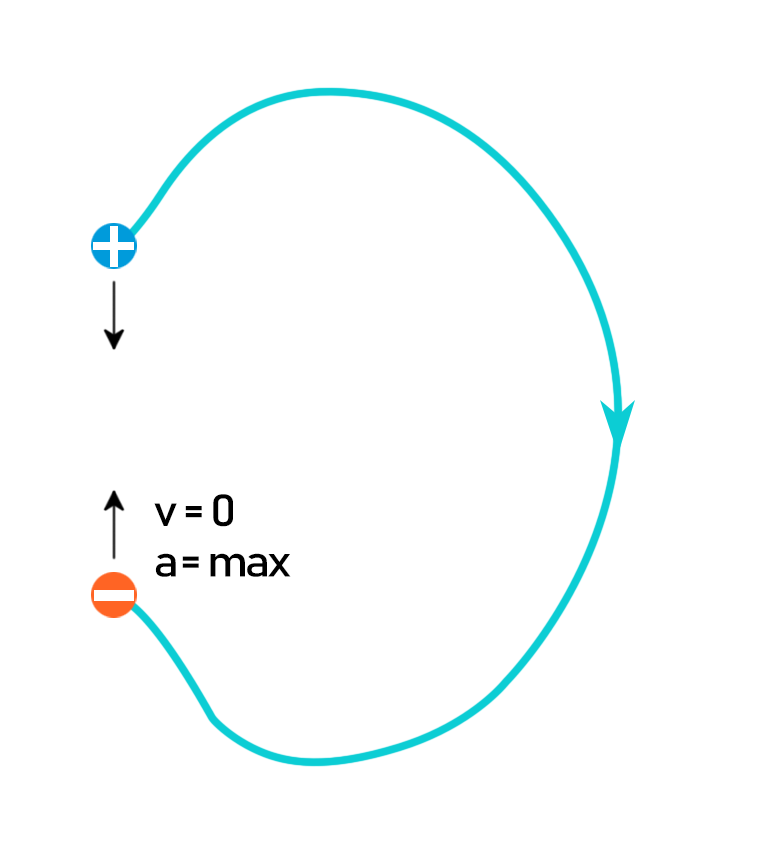
\includegraphics[width=5cm]{archivos/campos/campos1} % Tamaño de la imagen
		\caption{t = 0}
		\label{fig:campo1}
	\end{subfigure}
~ % Añadir el espacio deseado, si se deja la linea en blanco la siguiente subfigura ira en una nueva linea
	\begin{subfigure}[b]{0.3\textwidth} % Espacio horizontal ocupado por la subfigura
	\centering
		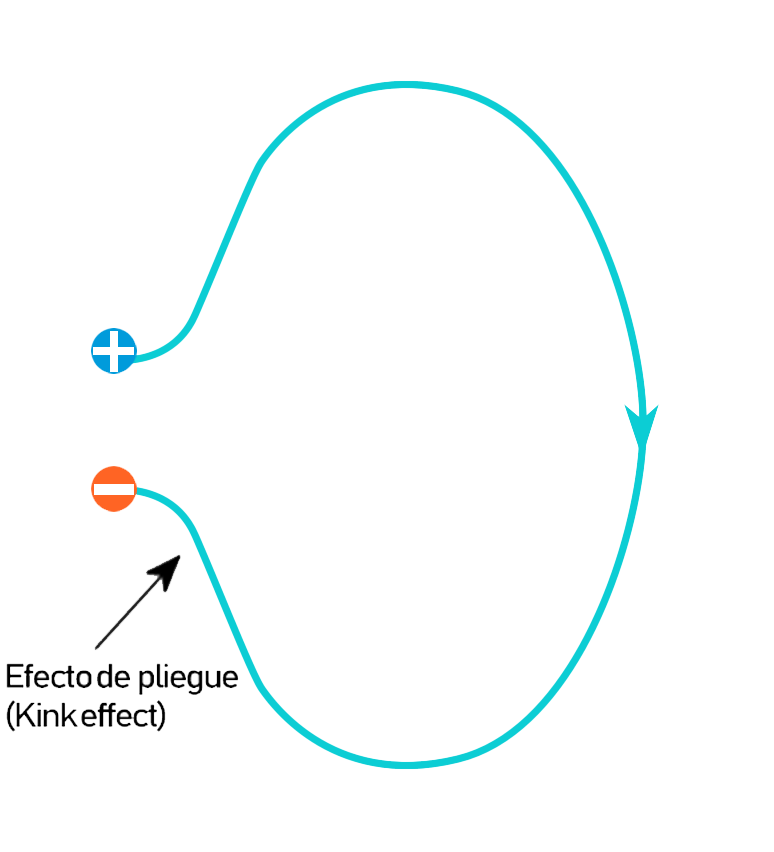
\includegraphics[width=5cm]{archivos/campos/campos2} % Tamaño de la imagen
		\caption{0 < t < T/4}
		\label{fig:campo2}
	\end{subfigure}
	\begin{subfigure}[b]{0.3\textwidth} % Espacio horizontal ocupado por la subfigura
	\centering
		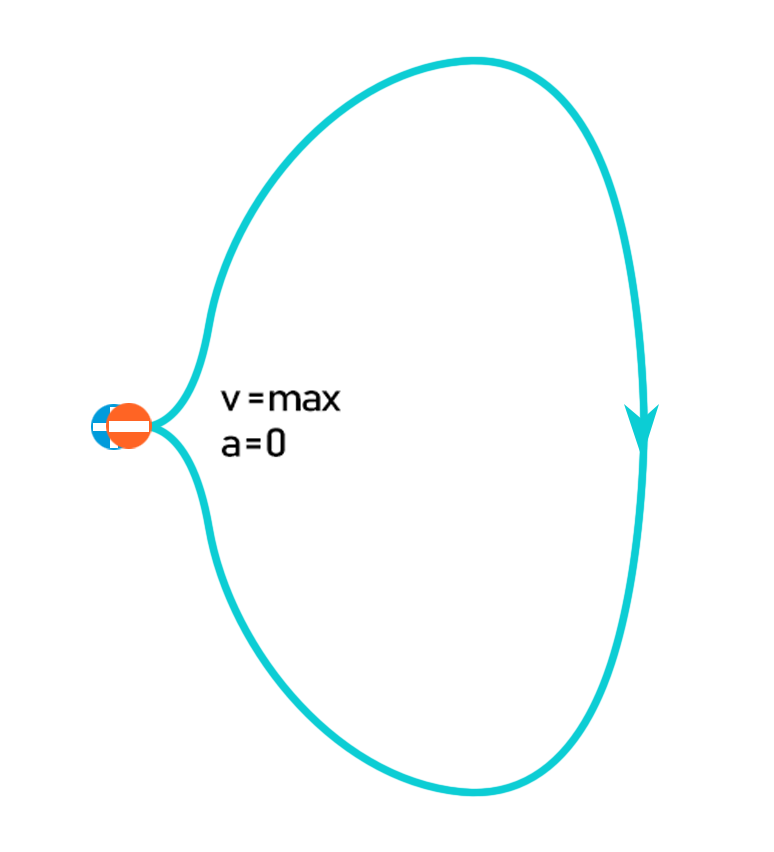
\includegraphics[width=5cm]{archivos/campos/campos3} % Tamaño de la imagen
		\caption{t = T/4}
		\label{fig:campo3}
	\end{subfigure}
	\begin{subfigure}[h]{0.5\textwidth} % Espacio horizontal ocupado por la subfigura
	\centering
	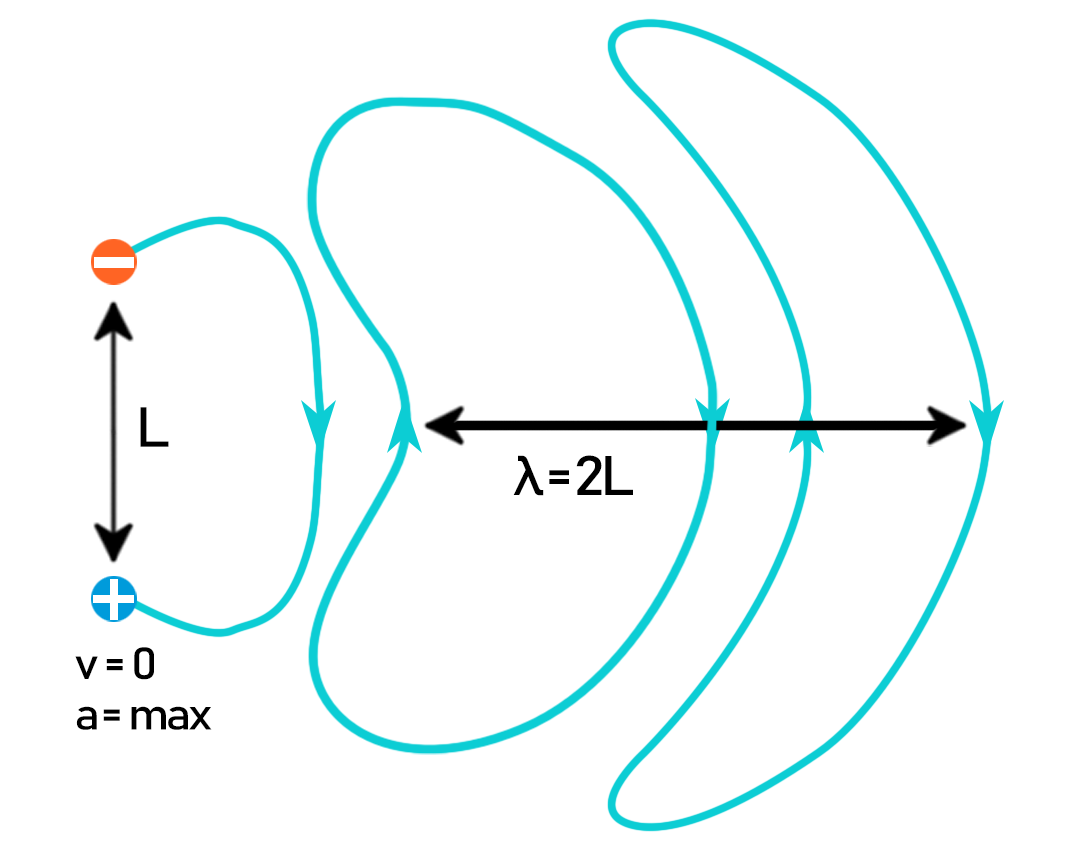
\includegraphics[width=10cm]{archivos/campos/campos4} % Tamaño de la imagen
	\caption{t > T/4}
	\label{fig:campo4}
\end{subfigure}
\caption{Proceso de separación de campo eléctrico}\label{sistemass}
\end{figure}

\par En la práctica se puede simular el experimento en lo que se denomina como antena dipolo, la antena más básica existente, que será estudiada con mayor detenimiento a lo largo de este capítulo. En una antena dipolo, al aplicar una tensión variable sobre los bornes de esta, las cargas irán oscilando de un extremo a otro según la polaridad del generador en ese instante, produciendo campos eléctricos capaces de separarse de la antena, con su consiguiente generación de campos magnéticos. El conjunto de la propagación de ambos campos son los campos electromagnéticos en los que se propagará la \gls{oem}. En la figura \ref{fig:dipolo} se pueden observar ejemplos de antenas dipolo. 

\begin{figure}[h]
\centering
	\begin{subfigure}[b]{0.4\textwidth} % Espacio horizontal ocupado por la subfigura
		\centering
		\includegraphics[width=7cm]{archivos/dipolo/dipole1} % Tamaño de la imagen
		\caption{Esquema de un dipolo}
		\label{fig:dipolo1}
	\end{subfigure}
~ % Añadir el espacio deseado, si se deja la linea en blanco la siguiente subfigura ira en una nueva linea
	\begin{subfigure}[b]{0.4\textwidth} % Espacio horizontal ocupado por la subfigura
	\centering
		\includegraphics[width=7cm]{archivos/dipolo/dipole2} % Tamaño de la imagen
		\caption{Dipolo instalado sobre un poste}
		\label{fig:dipolo2}
	\end{subfigure}
\caption{Antenas dipolo de media onda}\label{fig:dipolo}
\end{figure}

\par El principio básico de diseño de antenas se basa en la geometría de estas. Es importante remarcar que para que la transmisión de la señal aplicada por el generador y que se desea convertir en \gls{oem}, la longitud de los lados del dipolo deben estar relacionados con la longitud de onda de la señal que se desea transmitir. En el caso del dipolo, los extremos tendrán una longitud de $\lambda$/4. Al juntan ambos extremos se puede observar que la antena tendrá una dimensión total de $\lambda$/2, y si se tiene en cuenta que la longitud de onda de la \gls{oem} generada es el doble de la longitud de la antena, se obtendrá una \gls{oem} radiada cuya frecuencia sea idéntica a la aplicada por el generador.
\\
\par Aunque se ha analizado el caso de una antena para que funcione como transmisora, el mismo principio de funcionamiento se aplica cuando queremos que esta funcione como receptora de señales. Una \gls{oem} que viaje por el espacio será capaz de hacer oscilar las cargas de una antena receptora cuando su frecuencia y las longitud de la antena estén directamente relacionadas y se produzca la resonancia sobre esta. La diferencia es que a la salida de la antena receptora no tendremos un generador, sino lo que denominaremos como carga, pudiendo ser esta cualquier tipo de componente eléctrico o electrónico que sea capaz de trabajar con las corrientes eléctricas producidas por la fluctuación de cargas eléctricas en el interior de la antena.

\section{Caracterización de antenas}
\par Para saber qué tipo de antena se puede hacer más conveniente para un uso concreto se ha de tener en cuenta sus características. Las principales características de las antenas son:

\subsection{Polarización}
\par Como se hizo mención en el \todo{capitulo 1}, las \gls{oem} pueden estar polarizadas. Si se secciona a una \gls{oem} perpendicularmente a su vector de propagación y vemos el dibujo que va formando campo eléctrico en dicha sección conforme pasa el tiempo observaríamos qué tipo de polarización tiene la \gls{oem}. Las tres polarizaciones más comunes son: Lineal, circular y elíptica.

\begin{itemize}
\item\textbf{Polarización lineal: }Cuando se observa que la figura trazada por el campo eléctrico es una recta, se dirá que esta está polarizada linealmente. Analíticamente se producirá polarización lineal cuando las fases de las componentes ortogonales del campo eléctrico difieran en un múltiplo entero de $\pi$ radianes. La variación temporal de los campos eléctricos con polarización lineal se puede representar fasorialmente como:
\begin{equation}
	\vec{E} = \hat{x}e^{^{j(\omega t-kz)}}
	\label{eq:pollineal}
\end{equation}
\begin{figure}[h]
    \centering
        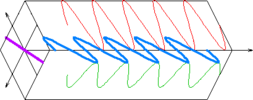
\includegraphics[width=6cm]{archivos/polarizacion/lineal}
        \caption{Onda electromagnética polarizada linealmente}
        \label{fig:pollin}
\end{figure}
\item\textbf{Polarización circular: }Cuando se observa que la figura trazada por el campo eléctrico es un círculo, se dirá que esta está polarizada circularmente. Analíticamente se producirá polarización circular cuando las fases de las componentes ortogonales del campo eléctrico sean $\pi$/2 o 3$\pi$/2 y las amplitudes sean iguales. La variación temporal de los campos eléctricos con polarización circular se puede representar fasorialmente como:

\begin{subequations}
	\begin{eqnarray}
		\vec{E} = (\hat{x}+j\hat{y})e^{^{j(\omega t-kz)}} \label{ecu:polcirlev} \\ % Salto de línea
		\vec{E} = (\hat{x}-j\hat{y})e^{^{j(\omega t-kz)}} \label{ecu:polcirdex} 
	\end{eqnarray}
\end{subequations}

\begin{figure}[h]
    \centering
        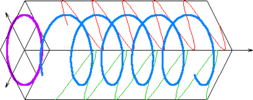
\includegraphics[width=6cm]{archivos/polarizacion/circular}
        \caption{Onda electromagnética polarizada circularmente}
        \label{fig:polcir}
\end{figure}

En este caso el signo que se encuentra en el interior de la suma de componentes indicará el sentido de giro en la polarización circular: Positivo será una rotación levógira y negativo una rotación dextrógira.

\item\textbf{Polarización elíptica: }Cuando se observa que la figura trazada por el campo eléctrico es una elipse, se dirá que esta está polarizada elípticamente. El resto de casos en los que la polarización no sea ni circular ni lineal serán polarizaciónes elípticas. La variación temporal de los campos eléctricos con polarización elíptica se puede representar fasorialmente como:

\begin{equation}
	\vec{E} = ((2+j)\hat{x}-3j\hat{y})e^{^{j(\omega t-kz)}}
	\label{eq:polelip}
\end{equation}
\begin{figure}[h]
    \centering
        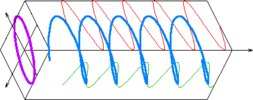
\includegraphics[width=6cm]{archivos/polarizacion/eliptica}
        \caption{Onda electromagnética polarizada elípticamente}
        \label{fig:poleli}
\end{figure}

\end{itemize}

\par En las ámbito de las radiocomunicaciones y en concreto de la telefonía móvil, la polarización más común en la que se emiten y reciben las \gls{oem} es la lineal-vertical. En otros casos como la transmisión de televisión se uriliza polarización lineal-horizontal. En comunicaciones vía satélite se alternan las polarizaciones lineales horizontales y verticales para reducir la interferencia entre señales que transmiten en el mismo rango de frecuencias.
\\
\par Se ha de tener en cuenta que cada antena se diseña para trabajar con una polarización concreta y las señales recibidas cuya polarización sea distinta a esta serán atenuadas debido al \textit{factor de pérdidas por polarización} ($C_{p}$):

\begin{equation}
	C_{p}=\left | \hat{u}_{tx}\cdot \hat{u}_{rx} \right |
	\label{eq:polarizationlossfactor}
\end{equation}

\par Donde $\hat{u}_{tx}$ es el vector unitario del campo eléctrico incidente y $\hat{u}_{rx}$ es el vector unitario del campo eléctrico de la antena receptora. 

\subsection{Impedancia}

\par Cualquier antenas se puede expresar como una carga en un circuito eléctrico, lo que facilita su análisis de impedancias, potencias y adaptación (fig. \ref{fig:impedancia}). Existen varios parámetros de impedancia que caracterizan a la antena. Por lo general, teniendo en cuenta la \textit{Ley de Ohm}, se define la impedancia de una antena como la relación entre la tensión y la corriente en los bornes de esta. 

\begin{equation}
	Z_{a}=\frac{V_{i}}{I_{i}}=R_{a}+jX_{a}
	\label{eq:impendaciaantena}
\end{equation}

\par Donde $R_{a}$ es la componente real u óhmica de la impedancia y $jX_{a}$ es la parte imaginaria o reactiva de la impedancia. La componente real puede ser a su vez descompuesta en dos términos: La resistencia de radiación y la resistencia óhmica o de pérdidas. La resistencia de radiación se define como la relación entre la potencia total radiada y la corriente eficaz en los terminales de la antena al cuadrado. La resistencia ohmica de la antena se define como la relación entre la potencia disipada debido a las pérdidas resistivas y la corriente que circula por sus terminales al cuadrado. Por otro lado la parte reactiva de la impedancia dependerá de sus dimensiones, la frecuencia de resonancia o el tipo de antena que estemos usando.

\begin{equation}
	Z_{a}=(R_{r}+R_{\Omega})+jX_{a}
	\label{eq:impendaciaantenatotal}
\end{equation}

\par Si se analizan las potencias según el tipo de resistencia, de radiación y óhmica, se obtiene que:

\begin{subequations}
	\begin{eqnarray}
		P_{r}=\frac{1}{2}\left | I_{o}  \right |^{2}R_{r} \label{ecu:potenciarad} \\ % Salto de línea
		P_{\Omega}=\frac{1}{2}\left | I_{o}  \right |^{2}R_{\Omega} \label{ecu:potenciaohm} 
	\end{eqnarray}
\end{subequations}

\begin{figure}[h]
    \centering
        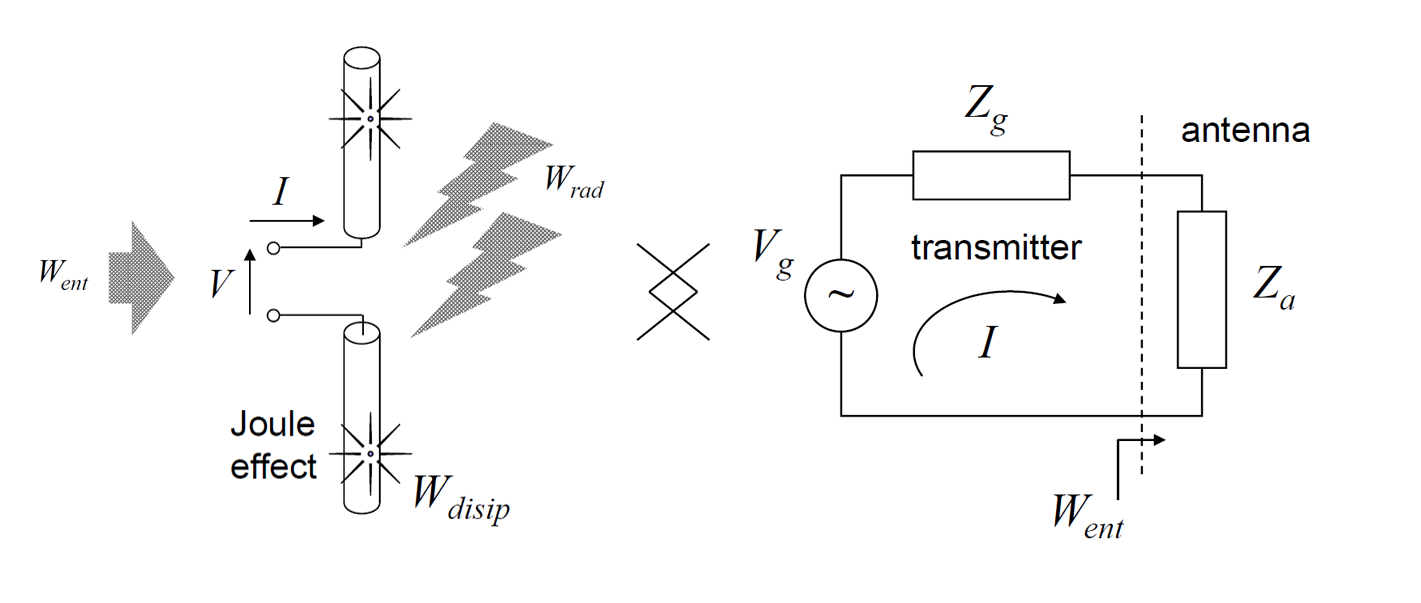
\includegraphics[width=15cm]{archivos/impedancia}
        \caption{Circuito equivalente de una antena transmisora}
        \label{fig:impedancia}
\end{figure}

\subsection{Diagrama de Radiación}

\par El diagrama de radiación es usado para representar gráficamente las propiedades de la radiación de una antena en un función de unas coordenadas angulares espacias, a una distancia fija. Para su representación se usan coordenadas esféricas o polares. Es una manera muy efectiva de conocer en qué direcciones concentra su radiación nuestra antena así como posibles radiaciones no deseadas que puedan existir un diseño particular. Para representar sobre un plano polar el diagrama de radiación aplicaremos la siguiente ecuación:

\begin{equation}
	t(\theta, \phi )=\frac{\left | E(r, \theta, \phi ) \right |^2}{\left | E_{max}(r) \right |^2}= \frac{P(r,\theta ,\phi)}{P_{max}(r)}
	\label{eq:diagramarad}
\end{equation}

\par El consistir en un plano de dos dimensiones: Angulo de radiación ($\theta$) e intensidad de radiación (t($\theta $, $\phi $)), debemos tener en cuenta que solo obtendremos el diagrama de radiación para un solo ángulo de transmisión de la antena. Es mediante el ángulo $\phi $ con el que podremos ir variando los resultados en el diagrama de radiación para poder observar como se propaga la antena en diferentes planos como son comúnmente el plano E y H (fig. \ref{fig:pattern}).

\begin{itemize}
\item \textbf{Plano E: }Es el plano donde podemos encontrar el vector del campo eléctrico y su dirección de máxima radiación (XZ). Este plano se encuentra en $\phi $ = 0º. 

\item \textbf{Plano E: }Es el plano donde podemos encontrar el vector del campo magnético y su dirección de máxima radiación (XY). Este plano se encuentra en $\phi $ = 90º.
\end{itemize}

\begin{figure}[h]
    \centering
        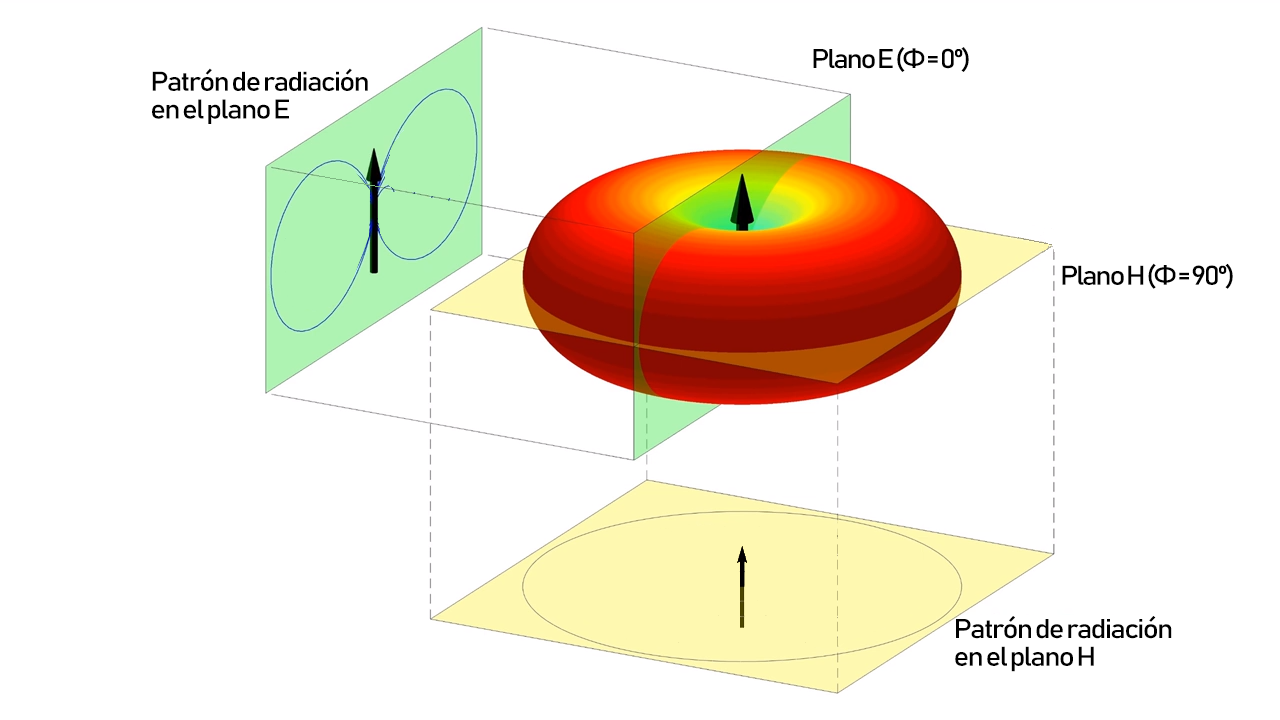
\includegraphics[width=15cm]{archivos/radiacion/pattern}
        \caption{Ejemplo de patrones de radiación en los planos E y H para antena dipolo}
        \label{fig:pattern}
\end{figure}

\par Existen ciertos parámetros que caracterizan a una antena que pueden ser localizados y calculados con facilidad gracias al diagrama de radiación tanto en coordenadas polares como en cartesianas (fig. \ref{fig:carte}). Estos parámetros son:

\begin{itemize}

\item \textbf{Lóbulos: }Son los haces de radiación. Se dividen en:
	\begin{itemize}
	\item \textbf{Lóbulo principal: }Se define siempre como la dirección de máxima radiación, siendo este siempre el haz con mayor intensidad de radiación.
	\item \textbf{Lóbulos secundarios: }Son los primeros haces de menor intensidad que aparecen en los laterales del lóbulo principal. 
	\item \textbf{Lóbulos menores: }Son el resto de haces de radiación los cuales son, normalmente, indeseados. Cuanto más directiva sea la antena, mayor será su número. 
	\item \textbf{Lóbulos trasero: }Es el haz de radiación que encontraremos siempre a 180º respecto al lóbulo principal. Normalmente, suele ser indeseado y su presencia puede producir interferencia con otras antenas del entorno así como una menor eficiencia para el propósito de nuestra antena.
	\end{itemize}	

\item \textbf{Ancho de haz a -3dB (HPBW)}: Se define como el ángulo recorrido por el lóbulo principal desde sus dos pasadas por -3dB de potencia, es decir, la mitad de la potencia máxima radiada. 

\item \textbf{Ancho de haz entre nulos (FNBW)}: Ángulo recorrido desde los dos nulos localizados a los laterales del lóbulo principal.

\item \textbf{Nivel de lóbulos laterales (SLL)}: Se define como la diferencia de niveles entre el nivel del lóbulo principal y el primer lóbulo secundario.

\item \textbf{Relación delante/atras (F/B)}: Diferencia de niveles entre el lóbulo principal y el trasero: 

\begin{equation}
	F/B(dB)=-10\log_{10}t(\theta+180^{\circ})
	\label{eq:fb}
\end{equation}

\end{itemize}

\begin{figure}[h]
    \centering
        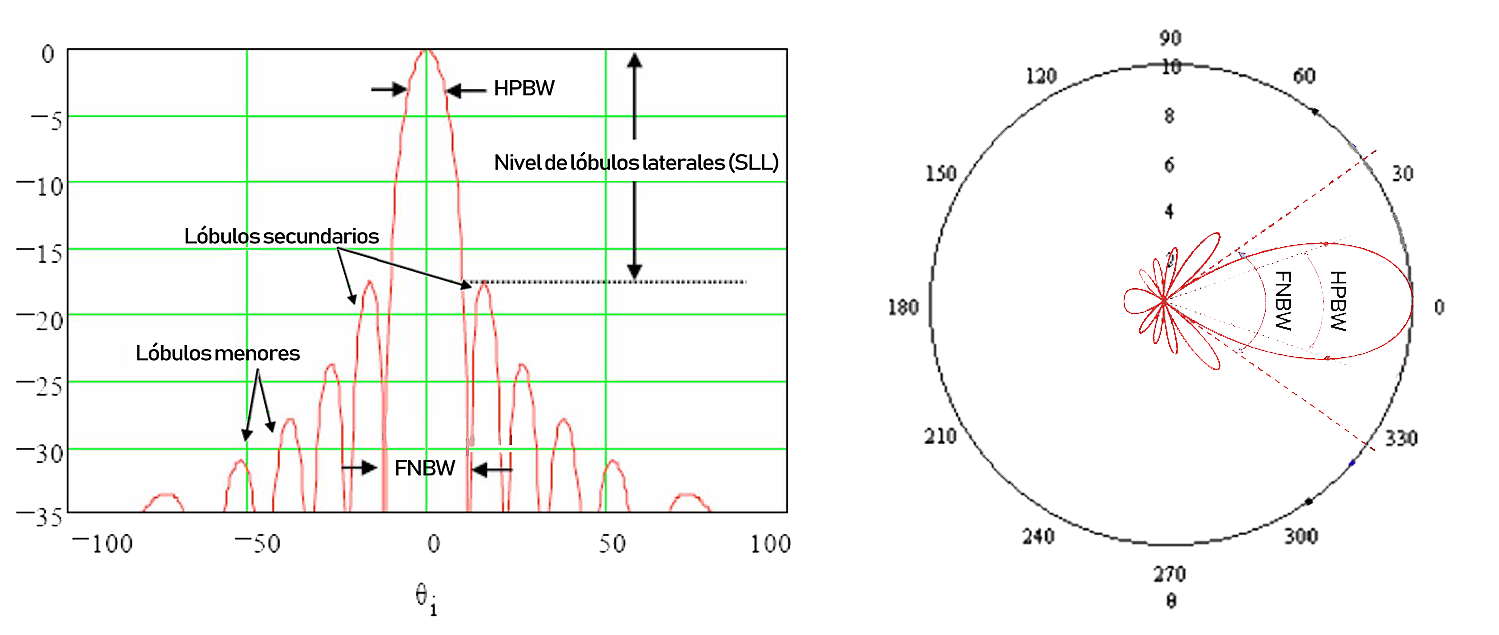
\includegraphics[width=15cm]{archivos/radiacion/pat3}
        \caption{Comparación de los parámetros del diagrama de radiación en planos cartesianos y polares}
        \label{fig:carte}
\end{figure}

\par Los patrones principales de radiación son:

\begin{itemize}
\item \textbf{Isotrópico: }La radiación de la antena fluye en todas las direcciones del espacio. Esta antena es completamente teórica ya que es imposible simular su patrón de directividad en una antena real. Se tiene como referencia para el cálculo de directividad de una antena.
\item \textbf{Omnidireccional: }Se dice que la antena es omnidireccional cuando el patrón de radiación es simétrico y equidistante en todos los ángulos del plano para uno o varios planos de radiación.
\item \textbf{Directiva: }Una antena es directiva cuando uno o varios de sus haces destacan sobre los demás. Esto puede ocurrir de manera intencionada, donde buscamos que el haz apunte hacia una dirección concreta, ej: Radioenlaces. O involuntariamente, cuando por ejemplo, tenemos lóbulos traseros o secundarios de bastante intensidad radiando a la vez que el principal. 
\end{itemize}

\begin{figure}[h]
    \centering
        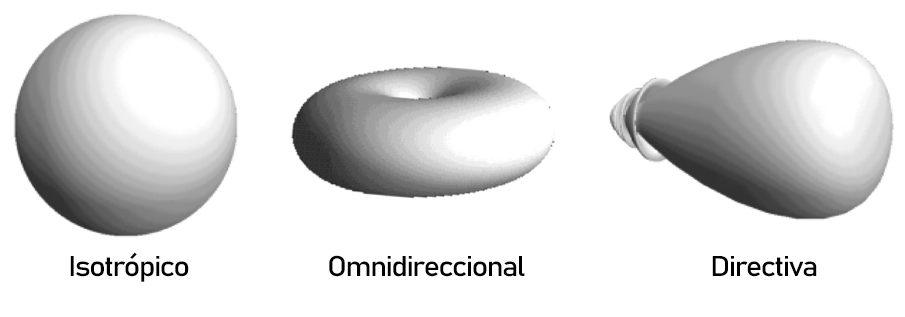
\includegraphics[width=15cm]{archivos/radiacion/patrones}
        \caption{Principales patrones de radiación}
        \label{fig:carte}
\end{figure}

\subsection{Directividad}

\par La directividad de una antena se define como la relación entre la intensidad de potencia de radiación en una dirección y distancia concretas, y la misma potencia radiada en caso de que la antena fuera isotrópica, es decir, cuya potencia radiada sea igual en todas las direcciones del espacio (eq. \ref{eq:directividad}). Este parámetro es muy importante para caracterizar la antena ya que nos representa la capacidad de una antena para concentrar la intensidad de radiación en una dirección determinada. Es posible obtener analíticamente el valor de directividad para un ángulo completo en el plano polar mediante:

\begin{equation}
	D(\theta, \phi )=\frac{P(r,\theta ,\phi)}{P_{iso}}= \frac{P(r,\theta ,\phi)}{\frac{W_{rad}}{4\pi r^{2}}}
	\label{eq:directividad}
\end{equation}

\par Si nos fijamos en el patrón de radiación de una antena, se dirá que esta es más directiva cuanto mayor sea el nivel de intensidad de un haz así como menor sea la anchura del mismo. Para el caso de las antenas directivas (D > 20dB), se puede obtener una directividad considerando que la radiación es uniforme sobre el ángulo sólido definido sobre el HPBW (Ancho de haz a -3dB) mediante la aproximación:

\begin{equation}
	D=\frac{4\pi}{\Delta \theta _{-3dB} \Delta \phi _{-3dB}}
	\label{eq:directividadaprox}
\end{equation}

\subsection{Ganancia}

\par La ganancia de una antena se define como la relación entre la intensidad radiada en una dirección concreta y la intensidad de radiación que se recibiría en caso de que la antena fuera isotrópica (eq. \ref{eq:ganancia}). Este parámetro se relaciona proporcionalmente con la directividad mediante la eficiencia de transmisión de la antena.(eq. \ref{eq:ganaciadirect})


\begin{subequations}
	\begin{eqnarray}
		G(\theta, \phi)=\frac{P(r,\theta, \phi)}{\frac{W_{ent}}{4\pi r^2}} \label{eq:ganancia} \\ % Salto de línea
		G(\theta, \phi)=\eta_{t} D(\theta, \phi) \label{eq:ganaciadirect}
	\end{eqnarray}
\end{subequations}


